% !TEX root = ../main.tex
% File: chapters_part1/chap3_1.tex
% Nội dung cho Phần 3.1: Word Embeddings

\section{Word Embeddings: Cuộc cách mạng Biểu diễn Đầu tiên}
\label{sec:word_embeddings}

Các phương pháp biểu diễn dựa trên tần suất như BoW hay TF-IDF, mặc dù hữu ích, lại mắc phải hai nhược điểm chí mạng:
\begin{enumerate}
    \item \textbf{Độ thưa thớt (Sparsity):} Chúng tạo ra các vector có số chiều khổng lồ và hầu hết là số 0.
    \item \textbf{Thiếu vắng ngữ nghĩa (Lack of Semantics):} Các vector này không hề nắm bắt được mối quan hệ ngữ nghĩa giữa các từ. Đối với BoW, hai từ "tốt" và "tuyệt vời" là hoàn toàn khác biệt, không có mối liên hệ nào.
\end{enumerate}

\textbf{Word Embeddings} (Nhúng từ) ra đời để giải quyết triệt để hai vấn đề trên. Đây là một tập hợp các kỹ thuật học máy có mục tiêu biểu diễn mỗi từ trong từ vựng bằng một \textbf{vector dày đặc (dense vector)} có số chiều tương đối thấp (thường từ 50 đến 300 chiều). Quan trọng hơn, các vector này được học sao cho chúng có thể nắm bắt được các mối quan hệ ngữ nghĩa và cú pháp giữa các từ.

Ý tưởng nền tảng của Word Embeddings dựa trên \textbf{Giả thuyết Phân bố (Distributional Hypothesis)} của Firth (1957), được tóm gọn trong câu nói nổi tiếng:
\begin{tcolorbox}[
    title=Giả thuyết Phân bố,
    colback=yellow!10!white, colframe=yellow!50!black, fonttitle=\bfseries
]
"You shall know a word by the company it keeps." (Bạn có thể hiểu một từ qua những từ thường đi cùng với nó.)
\end{tcolorbox}
Nói cách khác, những từ xuất hiện trong các ngữ cảnh tương tự nhau thì có khả năng mang ý nghĩa tương tự nhau. Word Embeddings là hiện thực hóa của giả thuyết này bằng các mô hình mạng nơ-ron.

\subsection{Lý thuyết Word2Vec: CBOW \& Skip-gram}
\label{ssec:word2vec}
Được giới thiệu bởi Tomas Mikolov và các cộng sự tại Google vào năm 2013 \cite{mikolov2013efficient, mikolov2013distributed}, Word2Vec không phải là một thuật toán duy nhất mà là một bộ công cụ bao gồm hai kiến trúc mô hình chính: \textbf{CBOW (Continuous Bag-of-Words)} và \textbf{Skip-gram}. Word2Vec đã tạo ra một cuộc cách mạng trong lĩnh vực Xử lý Ngôn ngữ Tự nhiên (NLP), dân chủ hóa việc sử dụng \textit{word embeddings} nhờ vào hiệu quả tính toán và chất lượng của vector biểu diễn mà nó tạo ra.

\subsubsection{Kiến trúc chung: Mạng Nơ-ron Nông}
\label{sssec:w2v_architecture}
Cốt lõi của Word2Vec là một ý tưởng đơn giản đến bất ngờ: thay vì xây dựng một mô hình ngôn ngữ phức tạp, chúng ta thiết kế một nhiệm vụ "giả" (fake task) và trong quá trình huấn luyện mô hình để giải quyết nhiệm vụ đó, chúng ta sẽ học được các vector từ chất lượng cao.

\paragraph{Nhiệm vụ "giả" so với Mô hình Ngôn ngữ "thật"}
Gọi là "giả" vì mục tiêu cuối cùng của chúng ta không phải là giải quyết tốt nhiệm vụ dự đoán từ, mà là học được ma trận trọng số \textbf{W}. Một mô hình ngôn ngữ "thật" (true language model), chẳng hạn như các mô hình dựa trên RNN, sẽ có mục tiêu phức tạp hơn nhiều: dự đoán từ tiếp theo dựa trên toàn bộ lịch sử các từ trước đó ($P(w_t | w_1, ..., w_{t-1})$). Việc này đòi hỏi kiến trúc sâu và phức tạp hơn.

Ngược lại, Word2Vec đơn giản hóa triệt để vấn đề: nó chỉ dự đoán từ dựa trên một cửa sổ ngữ cảnh cục bộ nhỏ. Sự đơn giản hóa này chính là chìa khóa thành công: nó cho phép mô hình xử lý hiệu quả một lượng dữ liệu văn bản khổng lồ. Gradient từ nhiệm vụ đơn giản này, tuy không hoàn hảo cho việc dự đoán ngôn ngữ, lại cực kỳ hiệu quả trong việc định hình một không gian vector mà ở đó các từ có ngữ cảnh tương tự được đặt gần nhau.

Cả CBOW và Skip-gram đều sử dụng kiến trúc mạng nơ-ron "nông" (shallow) chỉ với một lớp ẩn duy nhất. Giả sử từ vựng của chúng ta có \textbf{V} từ độc nhất và chúng ta muốn học các vector biểu diễn có \textbf{N} chiều (embedding dimension).

\begin{itemize}
    \item \textbf{Lớp vào (Input Layer):} Đầu vào là một vector \textit{one-hot} có kích thước $1 \times V$, đại diện cho một từ.
    \item \textbf{Lớp ẩn (Hidden Layer):} Không có hàm kích hoạt. Điểm mấu chốt nằm ở ma trận trọng số \textbf{W} kết nối lớp vào và lớp ẩn. Ma trận này có kích thước $V \times N$.
    \item \textbf{Lớp ra (Output Layer):} Ma trận trọng số \textbf{W'} kết nối lớp ẩn và lớp ra, có kích thước $N \times V$.
\end{itemize}

\begin{tcolorbox}[
    title=Ghi chú về Thiết kế Kiến trúc,
    colback=green!5!white, colframe=green!50!black, fonttitle=\bfseries
]
\textbf{1. Tại sao không có hàm kích hoạt ở lớp ẩn?} \\
Lớp ẩn của Word2Vec thực chất là một lớp tuyến tính (linear projection). Việc loại bỏ hàm phi tuyến (như ReLU hay Tanh) là một lựa chọn có chủ ý. Mục đích là để các mối quan hệ ngữ nghĩa (ví dụ: các phép loại suy -- analogies) có thể được biểu diễn dưới dạng các phép toán vector tuyến tính đơn giản (ví dụ: $\vec{v}_{\text{king}} - \vec{v}_{\text{man}} + \vec{v}_{\text{woman}} \approx \vec{v}_{\text{queen}}$). Nếu thêm hàm phi tuyến, cấu trúc tuyến tính này sẽ bị phá vỡ, làm cho các vector học được khó diễn giải và sử dụng hơn theo cách này. Lớp ẩn chỉ đóng vai trò như một bảng tra cứu (lookup table) để lấy ra vector embedding.

\textbf{2. Tại sao có hai ma trận trọng số W và W'?} \\
Mô hình có hai bộ vector cho mỗi từ:
\begin{itemize}
    \item \textbf{Input vectors (trong W):} Khi từ được dùng làm đầu vào (từ trung tâm trong Skip-gram, từ ngữ cảnh trong CBOW).
    \item \textbf{Output vectors (trong W'):} Khi từ được dùng làm mục tiêu dự đoán (từ ngữ cảnh trong Skip-gram, từ trung tâm trong CBOW).
\end{itemize}
Về mặt lý thuyết, việc có hai vai trò riêng biệt cho phép mô hình linh hoạt hơn. Sau khi huấn luyện xong, chúng ta thường chỉ sử dụng ma trận đầu vào \textbf{W} làm embedding cuối cùng. Đây là một quy ước phổ biến và cho kết quả tốt trong thực tế. Một số nghiên cứu cũng đề xuất các cách kết hợp khác (ví dụ, lấy trung bình cộng của hai vector tương ứng từ \textbf{W} và \textbf{W'}), nhưng chỉ dùng \textbf{W} vẫn là phương pháp tiêu chuẩn.
\end{tcolorbox}

Điều quan trọng là, chúng ta không thực sự quan tâm đến kết quả dự đoán của mạng. Mục tiêu cuối cùng của chúng ta là học được ma trận trọng số \textbf{W}. Sau khi huấn luyện, mỗi hàng của ma trận \textbf{W} chính là vector embedding N-chiều cho một từ tương ứng trong từ vựng. Do đó, \textbf{W} còn được gọi là \textbf{ma trận embedding (embedding matrix)}.

\begin{center}
    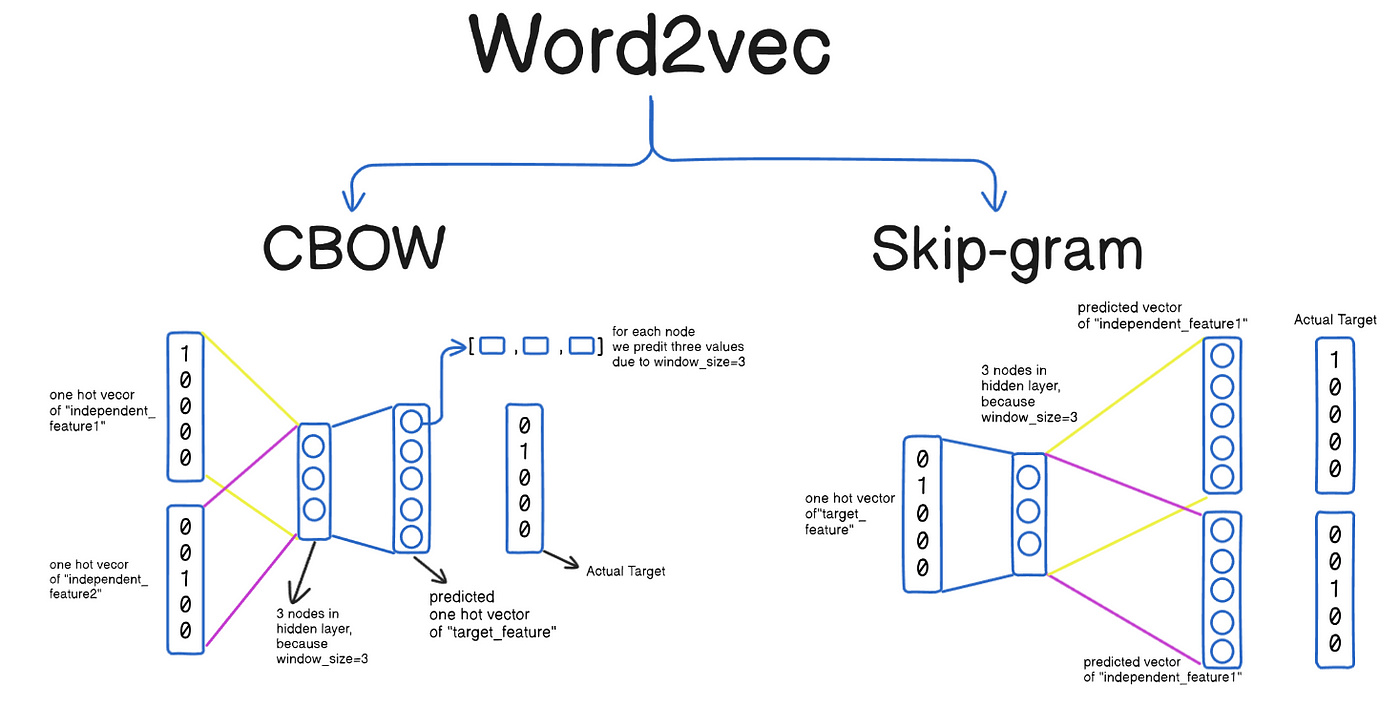
\includegraphics[width=0.8\textwidth]{word2vec_architecture.png}
    \captionof{figure}{Kiến trúc chung của Word2Vec. Khi nhân vector one-hot của một từ với ma trận $W$, thực chất chúng ta đang "chọn" ra hàng tương ứng với từ đó, chính là vector embedding của nó. Ma trận $W$ là mục tiêu chúng ta cần học.}
    \label{fig:word2vec_architecture}
\end{center}

\subsubsection{Mô hình CBOW (Continuous Bag-of-Words)}
\paragraph{Tư duy cốt lõi}
Mô hình CBOW hoạt động dựa trên giả định: "Một từ có thể được dự đoán bởi các từ xung quanh nó". Do đó, CBOW cố gắng \textbf{dự đoán một từ trung tâm (center word) dựa vào các từ ngữ cảnh (context words)}.

Ví dụ, trong câu "chú mèo [ngồi] trên chiếc chiếu" và cửa sổ ngữ cảnh là 2, CBOW sẽ lấy các từ ngữ cảnh \texttt{\{"chú", "mèo", "trên", "chiếc"\}} để dự đoán từ trung tâm là \texttt{\{"ngồi"\}}.

\paragraph{Cơ chế hoạt động}
\begin{enumerate}
    \item \textbf{Đầu vào:} Lấy các vector one-hot của các từ ngữ cảnh (ví dụ: \texttt{chú}, \texttt{mèo}, \texttt{trên}, \texttt{chiếc}).
    \item \textbf{Lấy vector embedding:} Từ ma trận embedding \textbf{W}, ta lấy ra các vector embedding tương ứng cho từng từ ngữ cảnh.
    \item \textbf{Tổng hợp ngữ cảnh:} Các vector embedding này được \textbf{lấy trung bình cộng} để tạo thành một vector ngữ cảnh duy nhất $\mathbf{v}_{\text{context}}$. Việc lấy trung bình này giải thích cho tên gọi "Bag-of-Words", vì nó làm mất đi thông tin về thứ tự các từ trong ngữ cảnh.
    \item \textbf{Dự đoán:} Vector $\mathbf{v}_{\text{context}}$ được nhân với ma trận \textbf{W'} và đưa qua hàm \textbf{softmax} để tạo ra một phân phối xác suất trên toàn bộ từ vựng. Vector đầu ra $\hat{\mathbf{y}}$ có kích thước $1 \times V$, trong đó phần tử thứ $j$ biểu diễn xác suất từ trung tâm là từ thứ $j$ trong từ vựng.
    \item \textbf{Huấn luyện:} So sánh vector xác suất dự đoán $\hat{\mathbf{y}}$ với vector one-hot $\mathbf{y}$ của từ trung tâm thực tế (từ \texttt{ngồi}). Hàm mất mát thường được sử dụng là \textbf{Cross-Entropy}, và lỗi được lan truyền ngược (backpropagation) để cập nhật các trọng số trong cả hai ma trận \textbf{W} và \textbf{W'}.
    $$ \mathcal{L} = -\sum_{j=1}^{V} y_j \log(\hat{y}_j) $$
\end{enumerate}

\paragraph{Phân tích lựa chọn thiết kế của CBOW}
Việc lấy trung bình các vector ngữ cảnh là một lựa chọn thiết kế vì sự đơn giản và hiệu quả tính toán. Nó không cần tham số nào để học và có thể được tính rất nhanh. Tuy nhiên, lựa chọn này có hai hệ quả quan trọng:
\begin{itemize}
    \item \textbf{Mất thông tin thứ tự:} CBOW không phân biệt được hai câu có cùng các từ ngữ cảnh nhưng khác trật tự. Trong nhiều tác vụ, việc mất thông tin cú pháp này là một hạn chế đáng kể.
    \item \textbf{"Lu mờ" từ hiếm:} Khi lấy trung bình, đóng góp của một vector từ hiếm có thể bị "lấn át" bởi các vector của các từ ngữ cảnh phổ biến hơn. Đây là lý do CBOW thường hoạt động kém hơn Skip-gram đối với các từ hiếm.
\end{itemize}
Các phương pháp phức tạp hơn như lấy trung bình có trọng số (dựa trên khoảng cách tới từ trung tâm) hoặc thậm chí dùng một cơ chế attention đơn giản có thể được xem xét, nhưng chúng sẽ làm tăng độ phức tạp và đi ngược lại triết lý "đơn giản, nhanh" của Word2Vec.

\subsubsection{Mô hình Skip-gram}
\paragraph{Tư duy cốt lõi}
Skip-gram đảo ngược lại nhiệm vụ của CBOW. Nó hoạt động dựa trên giả định: "Một từ có thể cho biết những từ nào sẽ xuất hiện xung quanh nó". Do đó, Skip-gram cố gắng \textbf{dự đoán các từ ngữ cảnh dựa vào một từ trung tâm}.

Ví dụ, với cùng câu trên, Skip-gram sẽ lấy từ trung tâm \texttt{\{"ngồi"\}} để cố gắng dự đoán từng từ trong tập ngữ cảnh \texttt{\{"chú", "mèo", "trên", "chiếc"\}}.

\paragraph{Cơ chế hoạt động}
Khác với CBOW, Skip-gram không gộp ngữ cảnh lại. Thay vào đó, nó tạo ra nhiều mẫu huấn luyện hơn từ một cửa sổ ngữ cảnh.
\begin{enumerate}
    \item \textbf{Đầu vào:} Lấy vector one-hot của từ trung tâm (ví dụ: \texttt{ngồi}).
    \item \textbf{Lấy vector embedding:} Lấy ra vector embedding $\mathbf{v}_{\text{center}}$ của từ trung tâm từ ma trận \textbf{W}.
    \item \textbf{Dự đoán:} Vector $\mathbf{v}_{\text{center}}$ được đưa thẳng đến lớp ra (nhân với \textbf{W'} và qua hàm softmax) để tạo ra một vector xác suất $\hat{\mathbf{y}}$.
    \item \textbf{Huấn luyện:} Quá trình này được lặp lại cho \textbf{từng từ trong ngữ cảnh}. Với mỗi cặp (\texttt{từ trung tâm}, \texttt{từ ngữ cảnh}), một hàm mất mát \textbf{Cross-Entropy} được tính toán giữa dự đoán $\hat{\mathbf{y}}$ và vector one-hot của từ ngữ cảnh thực tế. Tổng các lỗi từ tất cả các cặp được sử dụng để cập nhật trọng số qua backpropagation. Điều này giúp Skip-gram học được các biểu diễn tinh vi hơn, đặc biệt cho các từ hiếm, nhưng cũng tốn nhiều thời gian huấn luyện hơn.
\end{enumerate}

\begin{center}
    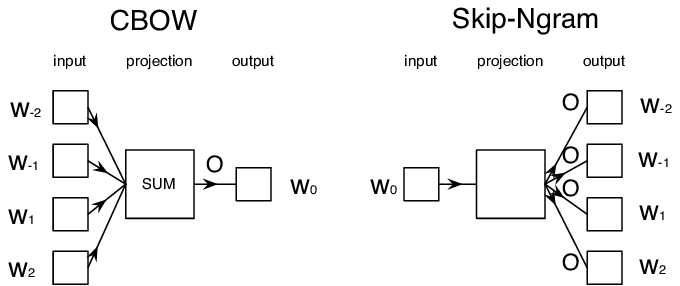
\includegraphics[width=0.9\textwidth]{cbow_skipgram_diagram.png}
    \captionof{figure}{So sánh trực quan giữa CBOW (tổng hợp ngữ cảnh để dự đoán 1 từ) và Skip-gram (dùng 1 từ để dự đoán nhiều từ trong ngữ cảnh, tạo thành các cặp huấn luyện riêng biệt).}
    \label{fig:cbow_skipgram_diagram}
\end{center}

\subsubsection{Vì sao Word2Vec học được ngữ nghĩa và gần--xa theo cosine?}
\label{sssec:w2v_why_semantics}

\paragraph{Nguyên lý phân bố (Distributional Hypothesis).}
Từ ngữ xuất hiện trong \emph{ngữ cảnh} giống nhau thường có nghĩa giống nhau. Khi huấn luyện Word2Vec để dự đoán từ--ngữ cảnh, các vector bị tối ưu sao cho những từ chia sẻ nhiều ngữ cảnh sẽ có \emph{hướng} gần nhau trong không gian.

\paragraph{CBOW: gom ngữ cảnh để dự đoán từ.}
Gọi $C$ là tập ngữ cảnh, $|C|=m$, $v_c \in \mathbb{R}^N$ là embedding của từ $c\in C$, và $u_w \in \mathbb{R}^N$ là vector ``ra'' cho từ trung tâm $w$. CBOW tính
\[
h \;=\; \frac{1}{m}\sum_{c\in C} v_c,\qquad 
p(w\,|\,C) \;=\; \mathrm{softmax}\big(u_w^\top h\big).
\]
Tối đa hoá $\log p(w\,|\,C)$ khiến $u_w^\top h$ tăng. Do $h$ là trung bình các $v_c$, mọi $v_c$ đều nhận gradient đẩy \emph{đồng hướng} với $u_w$. Khi hai từ $w_1,w_2$ thường cùng chia sẻ ngữ cảnh, các cập nhật lặp đi lặp lại làm $v_{w_1},v_{w_2}$ trở nên \emph{đồng hướng}.

\paragraph{Skip-gram với Negative Sampling (SGNS): kéo--đẩy cục bộ.}
Với cặp dương $(w,c)$ và các âm $n\in\mathcal{N}$, hàm mục tiêu một bước là
\[
\mathcal{L}_{\text{SGNS}} \;=\; 
- \log \sigma\!\big(u_c^\top v_w\big) \;-\; \sum_{n\in\mathcal{N}} \log \sigma\!\big(-u_n^\top v_w\big),
\]
trong đó $\sigma(x)=\frac{1}{1+e^{-x}}$. Gradient theo $v_w$ là
\[
\frac{\partial \mathcal{L}}{\partial v_w}
= \big(\sigma(u_c^\top v_w)-1\big)\,u_c \;+\; \sum_{n\in\mathcal{N}} \sigma(u_n^\top v_w)\,u_n.
\]
\emph{Trực giác:} với cặp dương, hệ số $\sigma(u_c^\top v_w)-1<0$ kéo $v_w$ \emph{tiến} về hướng $u_c$ (tăng tích vô hướng); với cặp âm, các hạng $+\sigma(u_n^\top v_w)\,u_n$ đẩy $v_w$ \emph{ra xa} các $u_n$. Qua thời gian, các từ chia sẻ ngữ cảnh dương sẽ bị kéo về \emph{cùng vùng} (gần nhau), còn các từ hiếm khi cùng ngữ cảnh sẽ bị \emph{đẩy xa}.

\paragraph{Vì sao cosine similarity?}
Huấn luyện tối ưu \emph{tích vô hướng} $u^\top v$ (do xuất hiện trong softmax/SGNS). Khi chuẩn hoá độ dài, tối đa hoá tích vô hướng tương đương tối đa hoá \emph{cosine}:
\[
u^\top v \;=\; \|u\|\,\|v\|\,\cos\theta.
\]
Trong thực tế, độ dài có thể dao động, nhưng \emph{hướng} mới mã hoá ``vị trí ngữ nghĩa''. Do đó, dùng cosine để đo gần--xa phản ánh đúng mục tiêu tối ưu hoá hướng.

\paragraph{Gần nghĩa, khác nghĩa, và trái nghĩa.}
\begin{itemize}
    \item \textbf{Gần nghĩa $\Rightarrow$ gần nhau:} nếu hai từ thường xuất hiện với \emph{cùng loại ngữ cảnh}, các cập nhật kéo chúng về \emph{đồng hướng} $\Rightarrow$ cosine cao.
    \item \textbf{Khác nghĩa $\Rightarrow$ xa nhau:} nếu hầu như không chia sẻ ngữ cảnh, vector bị các cập nhật khác hướng $\Rightarrow$ cosine thấp.
    \item \textbf{Trái nghĩa vẫn có thể gần nhau:} các cặp như \textit{nóng}--\textit{lạnh} xuất hiện trong \emph{ngữ cảnh hình thức} tương tự (``thời tiết \underline{nóng}/\underline{lạnh}'') nên vẫn bị kéo về gần nhau; Word2Vec không mô hình hoá \emph{độ phân cực nghĩa}. Muốn phân biệt polarity thường cần thêm tín hiệu (sentiment, lexicon, hoặc mô hình ngôn ngữ ngữ cảnh hoá).
\end{itemize}

\paragraph{Liên hệ lý thuyết: SGNS và Phân rã Ma trận PMI}
Một khám phá lý thuyết quan trọng của Levy và Goldberg \cite{levy2014neural} đã chỉ ra rằng mục tiêu tối ưu của Skip-gram với Negative Sampling (SGNS) thực chất tương đương với việc \textbf{phân rã ngầm định (implicit factorization)} một ma trận đặc biệt.  Cụ thể, hàm mục tiêu của SGNS hội tụ về việc tối ưu hóa sao cho:
\[ \mathbf{w}_i^\top \mathbf{c}_j \approx \text{PMI}(w_i, c_j) - \log k \]
trong đó $\mathbf{w}_i$ và $\mathbf{c}_j$ là các vector đầu vào và đầu ra, $k$ là số mẫu âm, và PMI (Pointwise Mutual Information) là một thước đo mức độ liên quan giữa hai từ:
\[ \text{PMI}(w, c) = \log \frac{P(w, c)}{P(w)P(c)} \]
Phát hiện này kết nối Word2Vec (một mô hình dự đoán, dựa trên mạng nơ-ron) với các phương pháp dựa trên đếm truyền thống (như LSA, GloVe) vốn trực tiếp phân rã ma trận đồng xuất hiện hoặc PMI. Nó cho thấy trực giác "kéo--đẩy" của SGNS không chỉ là một heuristic, mà là một cách hiệu quả để xấp xỉ một cấu trúc thống kê toàn cục của ngôn ngữ, làm sáng tỏ lý do tại sao các mối quan hệ ngữ nghĩa lại có thể được học một cách hiệu quả như vậy.

\paragraph{Hệ quả và giới hạn.}
\begin{itemize}
    \item \textbf{Tổng quát hoá theo ngữ cảnh:} ``nghĩa'' trong Word2Vec chủ yếu là \emph{tương đồng ngữ cảnh} (contextual co-occurrence).
    \item \textbf{Đa nghĩa:} một vector cho nhiều nghĩa sẽ trộn các ngữ cảnh (polysemy). Các mô hình \emph{ngữ cảnh hoá} (ELMo, BERT) khắc phục bằng vector phụ thuộc câu.
    \item \textbf{Cosine là thước đo mặc định:} vì hướng là tín hiệu chính của ``ngữ nghĩa'' đã học qua $u^\top v$.
\end{itemize}

\begin{tcolorbox}[title=Trực giác ``kéo--đẩy'' trong SGNS, colback=blue!5!white, colframe=blue!60!black, fonttitle=\bfseries]
\textbf{Kéo:} cặp dương $(w,c)$ làm tăng $u_c^\top v_w$ $\Rightarrow$ $v_w$ tiến về hướng $u_c$. 
\quad
\textbf{Đẩy:} cặp âm $(w,n)$ làm giảm $u_n^\top v_w$ $\Rightarrow$ $v_w$ rời xa hướng $u_n$.
\\[3pt]
Lặp lại trên toàn corpora tạo ra cấu trúc không gian nơi \emph{các trường ngữ cảnh} được biểu diễn bằng \emph{hướng vector}; cosine đo độ tương đồng các trường ngữ cảnh đó.
\end{tcolorbox}

\subsubsection{Thách thức tính toán và các kỹ thuật tối ưu hóa}
Cả hai mô hình đều đối mặt với một nút thắt cổ chai lớn: hàm \textbf{softmax} ở lớp ra. Việc tính toán mẫu số của hàm softmax đòi hỏi phải duyệt qua toàn bộ \textbf{V} từ trong từ vựng, cực kỳ tốn kém khi V có thể lên tới hàng triệu. Để giải quyết vấn đề này, hai kỹ thuật chính được đề xuất:

\paragraph{Subsampling và Cửa sổ ngữ cảnh động}
Trước khi đi vào các kỹ thuật tối ưu hóa chính, có hai thủ thuật quan trọng khác giúp cải thiện chất lượng embedding và tăng tốc độ huấn luyện:
\begin{itemize}
    \item \textbf{Subsampling các từ thường xuyên:} Các từ xuất hiện rất thường xuyên (như "là", "và", "trong" trong tiếng Việt, hay "the", "a" trong tiếng Anh) mang ít thông tin ngữ nghĩa đặc trưng. Chúng xuất hiện trong gần như mọi ngữ cảnh, do đó các cặp huấn luyện tạo ra từ chúng không giúp ích nhiều mà còn làm chậm quá trình huấn luyện. Subsampling là một kỹ thuật loại bỏ ngẫu nhiên các từ này trong quá trình tạo mẫu, với xác suất loại bỏ càng cao khi tần suất của từ càng lớn. Điều này giúp mô hình tập trung hơn vào các từ hiếm và quan trọng hơn.
    
    \item \textbf{Cửa sổ ngữ cảnh động (Dynamic Window):} Thay vì sử dụng một cửa sổ ngữ cảnh có kích thước cố định (ví dụ, luôn là 5), nhiều triển khai của Word2Vec sử dụng một kích thước cửa sổ động. Với mỗi từ trung tâm, một kích thước cửa sổ $C$ sẽ được chọn ngẫu nhiên trong khoảng từ 1 đến kích thước tối đa cho phép. Kỹ thuật này có tác dụng ngầm định là gán trọng số cao hơn cho các từ ngữ cảnh ở gần từ trung tâm, vì chúng có xác suất được lấy mẫu cao hơn các từ ở xa.
\end{itemize}

\paragraph{Negative Sampling}
Đây là kỹ thuật phổ biến hơn. Thay vì cập nhật trọng số cho toàn bộ từ vựng, ý tưởng là biến bài toán phân loại đa lớp (multi-class) thành một loạt các bài toán phân loại nhị phân (binary classification). Với mỗi cặp đầu vào (ví dụ, trong Skip-gram là \texttt{(từ trung tâm, từ ngữ cảnh)}):
\begin{enumerate}
    \item Chúng ta coi cặp này là một mẫu \textbf{dương tính (positive sample)}.
    \item Chúng ta lấy ngẫu nhiên \textbf{k} từ khác từ từ vựng (dựa trên một phân phối xác suất nhất định) và tạo ra \textbf{k} mẫu \textbf{âm tính (negative samples)}.
    \item Mô hình sẽ được huấn luyện để dự đoán đúng "nhãn" (1 cho mẫu dương tính, 0 cho các mẫu âm tính).
\end{enumerate}
Bằng cách này, trong mỗi bước cập nhật, chúng ta chỉ cần tính toán và cập nhật trọng số cho $k+1$ từ thay vì toàn bộ V từ, giúp tăng tốc độ huấn luyện lên rất nhiều.

\begin{tcolorbox}[
    title=Lựa chọn Thiết kế trong Negative Sampling,
    colback=orange!5!white, colframe=orange!60!black, fonttitle=\bfseries
]
\textbf{1. Phân phối lấy mẫu âm (The Sampling Distribution):} \\
Việc lấy mẫu các từ "âm tính" không phải là ngẫu nhiên đồng nhất trên toàn bộ từ vựng. Thay vào đó, Mikolov đề xuất sử dụng một phân phối Unigram đã được điều chỉnh, trong đó xác suất chọn một từ $w$ làm mẫu âm là:
\[ P(w) = \frac{f(w)^{3/4}}{\sum_{j=1}^{V} f(w_j)^{3/4}} \]
trong đó $f(w)$ là tần suất của từ $w$. Lũy thừa $3/4$ là một heuristic được chọn qua thực nghiệm.
\begin{itemize}
    \item Nếu dùng lũy thừa $1$ (theo tần suất thô), các từ rất phổ biến sẽ được chọn làm mẫu âm quá thường xuyên.
    \item Nếu dùng lũy thừa $0$ (phân phối đều), các từ hiếm sẽ được chọn thường xuyên một cách phi thực tế.
    \item Lũy thừa $3/4$ là một sự cân bằng hợp lý: nó làm giảm nhẹ tần suất của các từ phổ biến và tăng nhẹ tần suất của các từ hiếm, tạo ra các mẫu âm đa dạng và thách thức hơn cho mô hình.
\end{itemize}

\textbf{2. Số lượng mẫu âm (k):} \\
Tham số $k$ (số mẫu âm cho mỗi mẫu dương) thể hiện sự đánh đổi giữa chất lượng và tốc độ.
\begin{itemize}
    \item Với các tập dữ liệu nhỏ, $k$ lớn hơn (ví dụ: 5-20) thường cho kết quả tốt hơn vì mỗi mẫu dương cần nhiều ví dụ âm để mô hình học được ranh giới quyết định.
    \item Với các tập dữ liệu cực lớn, $k$ có thể nhỏ hơn (ví dụ: 2-5), vì mô hình đã thấy đủ đa dạng mẫu trong dữ liệu.
\end{itemize}
Giá trị của $k$ càng lớn, gradient càng ổn định nhưng chi phí tính toán cho mỗi bước cập nhật càng cao.
\end{tcolorbox}

\paragraph{Hierarchical Softmax}
Kỹ thuật này sử dụng một cây nhị phân (cụ thể là cây Huffman) để biểu diễn tất cả các từ trong từ vựng. Các từ thường xuyên xuất hiện sẽ có đường đi ngắn hơn trên cây. Thay vì dự đoán một từ, mô hình sẽ dự đoán một chuỗi các lựa chọn trái/phải để đi từ gốc đến lá của từ đó. Điều này giảm độ phức tạp tính toán từ $O(V)$ xuống còn $O(\log_2V)$.

\begin{tcolorbox}[
    title=So sánh CBOW và Skip-gram,
    colback=blue!5!white, colframe=blue!60!black, fonttitle=\bfseries
]
\begin{tabular}{p{0.45\linewidth} | p{0.45\linewidth}}
    \textbf{CBOW} & \textbf{Skip-gram} \\
    \hline
    Dự đoán từ trung tâm từ ngữ cảnh. & Dự đoán các từ ngữ cảnh từ từ trung tâm. \\
    \hline
    Nhanh hơn, chỉ một lần cập nhật cho mỗi cửa sổ ngữ cảnh. & Chậm hơn, phải cập nhật nhiều lần (mỗi từ trong ngữ cảnh). \\
    \hline
    Kém hiệu quả với từ hiếm do việc lấy trung bình làm “lu mờ” chúng. & Tốt hơn với từ hiếm vì mỗi từ vẫn tạo ra một cặp huấn luyện riêng. \\
    \hline
    Tốt cho các từ thường xuyên xuất hiện. & Thường tốt hơn với dữ liệu lớn và từ hiếm. \\
    \hline
    \textbf{Khi nào dùng?} Khi tốc độ là ưu tiên và dữ liệu rất lớn. & \textbf{Khi nào dùng?} Thường được ưa chuộng trong nghiên cứu vì chất lượng biểu diễn cao. \\
\end{tabular}
\end{tcolorbox}
Nhìn chung, Skip-gram thường được ưa chuộng hơn trong nghiên cứu.

\subsection{Lý thuyết GloVe: Ma trận Đồng xuất hiện}
\label{ssec:glove}

GloVe \cite{pennington2014glove} (\textit{Global Vectors for Word Representation}) được giới thiệu năm 2014 bởi các nhà nghiên cứu tại Stanford như một phương pháp học \textbf{word embeddings} dựa trên thống kê toàn cục của ngôn ngữ. 
Khác với Word2Vec (mô hình \textit{predictive}, học từ các ngữ cảnh cục bộ), GloVe là một mô hình \textit{count-based} được huấn luyện bằng tư duy tối ưu giống mô hình dự đoán, nhằm tận dụng cả thông tin toàn cục và cục bộ.

\paragraph{Tư duy cốt lõi}
Tần suất đồng xuất hiện giữa các từ mang ý nghĩa ngữ nghĩa quan trọng. Ví dụ: từ \textit{ice} và \textit{steam} đều đồng xuất hiện với \textit{water}, nhưng:
\begin{itemize}
    \item \textit{ice} đồng xuất hiện nhiều hơn với \textit{solid}, ít với \textit{gas}.
    \item \textit{steam} đồng xuất hiện nhiều hơn với \textit{gas}, ít với \textit{solid}.
\end{itemize}
So sánh tỉ lệ xác suất đồng xuất hiện giúp phân biệt nghĩa của các từ.

\begin{tcolorbox}[
    title=GloVe: Sự giao thoa giữa Count-based và Predictive,
    colback=green!5!white, colframe=green!50!black, fonttitle=\bfseries
]
Một câu hỏi thường gặp là: Nếu GloVe xây dựng trên ma trận đếm toàn cục, tại sao nó không đơn giản là phân rã ma trận đó (như LSA)? Và nếu hàm mất mát của nó trông giống một bài toán dự đoán, tại sao nó không phải là mô hình predictive như Word2Vec?

Câu trả lời nằm ở chỗ GloVe kết hợp những điểm mạnh của cả hai phương pháp:
\begin{itemize}
    \item \textbf{Tận dụng thống kê toàn cục (Count-based):} Bằng cách tiền tính toán ma trận đồng xuất hiện $X$, GloVe có cái nhìn bao quát về toàn bộ kho văn bản ngay từ đầu. Mọi thông tin về tần suất và sự đồng xuất hiện đều được mã hóa trong ma trận này.
    \item \textbf Tối ưu hóa hiệu quả (Predictive-style): Thay vì thực hiện các phép phân rã ma trận phức tạp và tốn kém (như SVD trong LSA), GloVe định nghĩa một hàm mất mát dạng "hồi quy có trọng số". Mô hình sau đó học các vector bằng cách tối ưu hàm mất mát này trên từng cặp $(i, j)$ không rỗng trong ma trận $X$. Cách học lặp đi lặp lại trên các mẫu riêng lẻ này rất giống với tinh thần của các mô hình dự đoán, giúp việc huấn luyện trở nên hiệu quả và có thể song song hóa.
\end{itemize}
Do đó, GloVe có thể được xem là một mô hình "lai": nó trực tiếp tối ưu hóa để học các vector sao cho chúng có thể tái tạo lại được các thống kê toàn cục của ngôn ngữ.
\end{tcolorbox}

\paragraph{Tỉ lệ xác suất}
Cho từ $i$, $j$ và từ ngữ cảnh $k$, xác suất đồng xuất hiện được định nghĩa:
\[
P_{ik} = \frac{\text{số lần từ $k$ xuất hiện gần $i$}}{\text{tổng số lần xuất hiện ngữ cảnh của $i$}}
\]
GloVe chỉ ra rằng \textbf{tỉ lệ} $\frac{P_{ik}}{P_{jk}}$ chứa thông tin ngữ nghĩa: nếu $k$ liên quan nhiều đến $i$ hơn $j$, tỉ lệ này sẽ lớn.

\paragraph{Từ Tỉ lệ đến Tích vô hướng: Cầu nối Toán học}
Đây là bước nhảy vọt tinh tế nhất của GloVe. Các tác giả đã lập luận như sau:
\begin{enumerate}
    \item Mối quan hệ giữa ba từ $i, j, k$ được thể hiện qua tỉ lệ $P_{ik}/P_{jk}$. Mối quan hệ này nên được mô hình hóa bởi các vector của chúng: $w_i, w_j, w_k$. Ta có thể bắt đầu với một hàm tổng quát $F$:
    \[ F(w_i, w_j, w_k) = \frac{P_{ik}}{P_{jk}} \]
    \item Để mã hóa thông tin trong không gian vector tuyến tính, các tác giả đề xuất rằng $F$ nên chỉ phụ thuộc vào hiệu của hai từ đầu tiên, $F(w_i - w_j, w_k)$. Điều này giúp nắm bắt các mối quan hệ loại suy (analogy).
    \item Để đơn giản hóa hơn nữa, họ nhận thấy rằng vế phải là một đại lượng vô hướng, trong khi vế trái là một hàm của các vector. Cách tự nhiên nhất để biến các vector thành vô hướng là dùng tích vô hướng. Điều này dẫn đến:
    \[ F(w_i - w_j, w_k) \rightarrow (w_i - w_j)^\top w_k = w_i^\top w_k - w_j^\top w_k \]
    \item Kết hợp các bước trên và một vài biến đổi toán học (sử dụng tính chất của hàm đồng cấu giữa nhóm cộng và nhân), họ đi đến kết luận rằng một dạng hàm phù hợp là:
    \[ w_i^\top w_k \approx \log(P_{ik}) = \log(X_{ik}) - \log(X_i) \]
    Trong đó $X_{ik}$ là số lần $k$ xuất hiện trong ngữ cảnh của $i$, và $X_i$ là tổng số lần các từ xuất hiện trong ngữ cảnh của $i$.
    \item Hạng tử $\log(X_i)$ không phụ thuộc vào $k$. Nó có thể được gộp vào một số hạng bias $b_i$. Tương tự, để giữ tính đối xứng, một bias $b_k$ cũng được thêm vào cho từ ngữ cảnh. Điều này dẫn đến công thức mục tiêu cuối cùng, chính là nền tảng cho hàm mất mát của GloVe.
\end{enumerate}
Quá trình này cho thấy công thức mục tiêu không phải là ngẫu nhiên, mà là kết quả của một chuỗi lập luận chặt chẽ nhằm mã hóa các tỉ lệ thống kê vào một cấu trúc vector tuyến tính.

\paragraph{Cơ chế hoạt động}
\begin{enumerate}
    \item \textbf{Xây dựng ma trận đồng xuất hiện $X$:} 
    Duyệt toàn bộ kho văn bản, xây dựng ma trận $X \in \mathbb{R}^{V \times V}$ với:
    \[
    X_{ij} = \text{số lần từ $j$ xuất hiện trong ngữ cảnh của $i$}.
    \]
    \textit{Ngữ cảnh} thường được định nghĩa bởi một cửa sổ từ nhất định (window size).

    \item \textbf{Mục tiêu tối ưu:} 
    Ta muốn tìm vector từ $w_i, w_j \in \mathbb{R}^d$ và bias $b_i, b_j$ sao cho:
    \[
    w_i^\top w_j + b_i + b_j \approx \log X_{ij}.
    \]
    Lý do dùng $\log$ là vì tần suất đồng xuất hiện phân bố lệch (long-tailed), logarit giúp “nén” khoảng giá trị.

    \item \textbf{Hàm mất mát:}
    \begin{equation}
        J = \sum_{i,j=1}^{V} f(X_{ij}) \left( w_i^\top w_j + b_i + b_j - \log X_{ij} \right)^2
        \label{eq:glove_loss}
    \end{equation}
    Trong đó, $f(X_{ij})$ là hàm trọng số:
    \[
    f(x) = \begin{cases}
        (x/x_{\max})^\alpha & \text{nếu } x < x_{\max},\\
        1 & \text{nếu } x \ge x_{\max}
    \end{cases}
    \]
    với $\alpha \approx 0.75$ và $x_{\max}$ thường khoảng $100$. 
    Hàm này giảm ảnh hưởng của cặp từ xuất hiện quá thường xuyên và bỏ qua nhiễu từ cặp quá hiếm.

    \item \textbf{Kết quả:} 
    Sau khi tối ưu, tích vô hướng $w_i^\top w_j$ xấp xỉ log xác suất đồng xuất hiện, nghĩa là khoảng cách giữa các vector phản ánh mối quan hệ thống kê toàn cục của ngôn ngữ.
\end{enumerate}

\begin{tcolorbox}[
    title=Giải mã Hàm mất mát của GloVe,
    colback=orange!5!white, colframe=orange!60!black, fonttitle=\bfseries
]
Mỗi thành phần trong hàm mất mát của GloVe đều có một vai trò quan trọng và được lựa chọn cẩn thận:
\begin{itemize}
    \item \textbf{Vai trò của Logarit ($\log X_{ij}$):} Tần suất đồng xuất hiện $X_{ij}$ có phân bố trải dài trên nhiều bậc độ lớn (từ 1 đến hàng triệu). Việc lấy logarit giúp "nén" khoảng giá trị này lại. Điều này ngăn các cặp từ có tần suất cực lớn (ví dụ: "the" và "is") tạo ra một giá trị lỗi quá lớn và lấn át hoàn toàn đóng góp của các cặp từ hiếm nhưng mang nhiều ý nghĩa.

    \item \textbf{Ý nghĩa của các Bias ($b_i, b_j$):} Các số hạng bias này không chỉ là một kỹ thuật thông thường. Chúng giúp hấp thụ các hiệu ứng chính (main effects) liên quan đến tần suất. Cụ thể, $b_i$ có thể học để mã hóa sự "nổi tiếng" chung của từ $i$ (một từ rất phổ biến sẽ có $X_{ij}$ lớn với nhiều từ $j$). Bằng cách để các bias xử lý phần thông tin này, vector chính $w_i$ và $w_j$ có thể tập trung hơn vào việc mã hóa mối quan hệ tương tác ngữ nghĩa giữa hai từ, làm cho các vector trở nên "trong sáng" hơn.
    
    \item \textbf{Tại sao cần hàm trọng số $f(X_{ij})$?}: Đây là thành phần quan trọng nhất, giải quyết hai vấn đề lớn:
    \begin{enumerate}
        \item \textbf{Các cặp có $X_{ij} = 0$:} Có vô số cặp từ không bao giờ đồng xuất hiện. Nếu không có $f(X_{ij})$, chúng ta sẽ phải tính tổng trên tất cả $V \times V$ cặp, và $\log(0)$ là không xác định. Hàm trọng số được thiết kế sao cho $f(0) = 0$, giúp loại bỏ hoàn toàn các cặp này khỏi hàm mất mát một cách tự nhiên.
        \item \textbf{Giảm trọng số các cặp quá phổ biến:} Các cặp từ đồng xuất hiện rất thường xuyên (ví dụ: "it is", "of the") thường mang ít thông tin ngữ nghĩa đặc biệt. Dù đã có logarit, chúng vẫn có thể thống trị quá trình huấn luyện. Hàm $f(x)$ với $\alpha < 1$ (thường là 0.75) và ngưỡng $x_{\text{max}}$ đảm bảo rằng các cặp này không có trọng số quá lớn, cho phép mô hình quan tâm hơn đến các cặp từ hiếm hơn nhưng thú vị hơn về mặt ngữ nghĩa.
    \end{enumerate}
\end{itemize}
\end{tcolorbox}

\paragraph{Điểm mạnh và hạn chế}
\begin{itemize}
    \item \textbf{Ưu điểm:} 
    \begin{itemize}
        \item Kết hợp thông tin toàn cục (thống kê đồng xuất hiện) và cục bộ (tối ưu vector).
        \item Huấn luyện nhanh hơn Word2Vec trên dữ liệu lớn vì sử dụng ma trận đồng xuất hiện tiền tính toán.
        \item Vector tạo ra ổn định hơn với nhiều lần train.
    \end{itemize}
    \item \textbf{Hạn chế:}
    \begin{itemize}
        \item Yêu cầu lưu trữ ma trận đồng xuất hiện rất lớn khi từ vựng lớn.
        \item Không sinh embedding phụ thuộc ngữ cảnh (mỗi từ một vector cố định).
    \end{itemize}
\end{itemize}

\subsection{Lý thuyết FastText: Biểu diễn Subword}
\label{ssec:fasttext}

FastText được phát triển bởi nhóm Facebook AI Research (FAIR) năm 2017 \cite{bojanowski2017enriching}, nhằm khắc phục một hạn chế quan trọng của các mô hình như Word2Vec và GloVe: \textbf{không xử lý được các từ ngoài từ vựng} (Out-of-Vocabulary - OOV).  
Trong Word2Vec/GloVe, mỗi từ được coi như một “đơn vị nguyên tử” (atomic unit), và nếu từ đó không xuất hiện trong quá trình huấn luyện thì mô hình hoàn toàn không có vector cho nó.  

\paragraph{Tư duy cốt lõi}
Thay vì gán mỗi từ một vector duy nhất, FastText biểu diễn từ như một \textbf{tập hợp các n-gram ký tự} (\textit{bag of character n-grams}). Điều này cho phép mô hình:
\begin{itemize}
    \item Tận dụng thông tin cấu trúc hình thái (morphology) của từ.
    \item Sinh vector cho từ mới dựa trên các thành phần subword quen thuộc.
\end{itemize}

\paragraph{Cơ chế hoạt động}
\begin{enumerate}
    \item \textbf{Phân rã từ thành n-gram ký tự:}  
    Với kích thước $n=3$ (3-gram), từ \textit{sách} sẽ được bao quanh ký hiệu biên giới từ và phân rã thành:
    \[
    \langle s, \quad sa, \quad sác, \quad ách, \quad ch\rangle
    \]
    Ngoài ra, chính từ hoàn chỉnh \textit{sách} cũng được coi là một n-gram.  
    Ký hiệu \verb|<| và \verb|>| đánh dấu bắt đầu và kết thúc từ để phân biệt tiền tố/hậu tố.

    \item \textbf{Học embedding cho subword:}  
    FastText học một vector embedding cho \textbf{mỗi} n-gram ký tự, không chỉ cho từ hoàn chỉnh.

    \item \textbf{Tạo vector từ:}  
    Vector biểu diễn từ $w$ là trung bình (hoặc tổng) các vector embedding của tất cả các subword của $w$:
    \[
    \mathbf{v}(w) = \frac{1}{|G_w|} \sum_{g \in G_w} \mathbf{z}_g
    \]
    trong đó:
    \begin{itemize}
        \item $G_w$ = tập các n-gram ký tự của $w$.
        \item $\mathbf{z}_g$ = embedding của n-gram $g$.
    \end{itemize}

    \item \textbf{Huấn luyện:}  
    Về kiến trúc, FastText vẫn sử dụng Skip-gram (hoặc CBOW) như Word2Vec, nhưng thay vì ánh xạ từ $\rightarrow$ vector, nó ánh xạ tập hợp subword $\rightarrow$ vector.
\end{enumerate}

\begin{tcolorbox}[
    title=Ghi chú sâu về Biểu diễn Subword,
    colback=green!5!white, colframe=green!50!black, fonttitle=\bfseries
]
\textbf{1. Tại sao vẫn giữ vector cho từ hoàn chỉnh?} \\
Việc giữ lại vector cho cả từ gốc (ví dụ, embedding cho `<s>sách</s>`) bên cạnh các n-gram của nó là một lựa chọn thiết kế quan trọng. Vector của từ hoàn chỉnh đóng vai trò như một "mỏ neo", mang ý nghĩa tổng thể và giúp phân biệt các từ có chung nhiều n-gram nhưng nghĩa lại khác nhau. Nếu không có nó, các từ ngắn và có cấu trúc tương tự (ví dụ: `sun` và `sin`) có thể trở nên quá gần nhau trong không gian vector. Vector của từ hoàn chỉnh đảm bảo mỗi từ có một "danh tính" riêng biệt.

\textbf{2. Tại sao lấy trung bình thay vì các phép toán khác?} \\
Lấy trung bình là một cách đơn giản và hiệu quả để kết hợp các vector subword.
\begin{itemize}
    \item \textbf{So với Tổng (Sum):} Việc lấy trung bình giúp chuẩn hóa độ dài của vector từ. Nếu dùng tổng, các từ dài (có nhiều n-gram hơn) sẽ có xu hướng tạo ra các vector có độ lớn (norm) cao hơn, điều này có thể không mong muốn.
    \item \textbf{So với các cơ chế phức tạp hơn (Attention):} Mặc dù attention có thể học cách gán trọng số khác nhau cho các subword (ví dụ, gốc từ quan trọng hơn hậu tố), nó sẽ làm tăng đáng kể độ phức tạp tính toán, đi ngược lại triết lý "nhanh" (fast) của FastText.
\end{itemize}

\textbf{3. Quản lý bộ nhớ với Hashing Trick} \\
Số lượng n-gram ký tự có thể là cực lớn. Để giữ cho mô hình có kích thước hợp lý, FastText không lưu một vector cho mỗi n-gram duy nhất. Thay vào đó, nó sử dụng một hàm băm (hashing function) để ánh xạ mỗi n-gram vào một trong số $B$ "bucket" (thường $B$ khoảng 2 triệu). Tất cả các n-gram rơi vào cùng một bucket sẽ chia sẻ cùng một vector embedding. Kỹ thuật này giúp kiểm soát chặt chẽ bộ nhớ, dù có thể xảy ra xung đột (hai n-gram khác nhau cùng được ánh xạ vào một bucket), nhưng trong thực tế với một không gian băm đủ lớn, ảnh hưởng tiêu cực là không đáng kể.
\end{tcolorbox}

\paragraph{Ưu điểm nổi bật}
\begin{itemize}
    \item \textbf{Xử lý OOV:} Với từ mới chưa từng thấy, mô hình vẫn sinh được vector bằng cách cộng/trung bình embedding của các subword đã biết.
    \item \textbf{Hiểu hình thái:} Các từ cùng gốc hoặc chia sẻ tiền tố/hậu tố sẽ có embedding gần nhau.  
    Ví dụ: \textit{running}, \textit{runner}, \textit{runs} cùng chứa n-gram \verb|run|.
\end{itemize}

\paragraph{Hạn chế}
\begin{itemize}
    \item Kích thước mô hình lớn hơn do phải lưu embedding cho nhiều n-gram.
    \item Không xử lý được ý nghĩa phụ thuộc ngữ cảnh (mỗi từ vẫn một vector tĩnh).
    \item \textbf{Vấn đề từ đồng âm và sự trùng hợp ngẫu nhiên:} FastText không giải quyết được vấn đề đa nghĩa. Tệ hơn, nó có thể tạo ra các mối liên hệ sai lệch. Hai từ hoàn toàn không liên quan về nghĩa nhưng tình cờ có chung các n-gram ký tự (ví dụ, `pain` và `Spain` đều chứa `ain`) có thể bị đẩy lại gần nhau một cách không mong muốn trong không gian embedding.

    \item \textbf{Hiệu quả phụ thuộc vào đặc tính ngôn ngữ:} Phương pháp dựa trên n-gram ký tự hoạt động đặc biệt hiệu quả với các ngôn ngữ có hình thái học phong phú (như tiếng Đức, Thổ Nhĩ Kỳ, Phần Lan), nơi cấu trúc subword thực sự mã hóa thông tin ngữ pháp. Tuy nhiên, với các ngôn ngữ đơn lập như tiếng Việt hoặc các ngôn ngữ dùng hệ chữ tượng hình như tiếng Trung, lợi ích từ việc phân rã ký tự có thể ít rõ rệt hơn so với việc phân tích ở cấp độ từ hoặc âm tiết.
\end{itemize}

